\chapter*{Résumé}
La génération automatique de terrains virtuels est un problème sur lequel
planchent souvent les graphistes et les games designers, car pouvoir créer
 un monde virtuel persistant est une brique de base à de nombreuses
applications. Mais, même si le sujet a été maintes fois traité, il reste un
problème difficile non seulement techniquement à cause de la masse de calculs
 que cela représente mais aussi parce que le rendu final du paysage doit
paraître un tant soit peu réaliste aux yeux des utilisateurs.\\

Le but de ce projet est de créer une bibliothèque permettant la création de
terrains virtuels à partir de méthodes fractales. L'utilisateur de la bibliothèque
pourra réaliser des cartes carrées ou sphériques et disposera d'un choix
conséquent d'algorithmes de génération qui seront détaillés dans ce rapport.
La bibliothèque permettra aussi la visualisation des terrains avec différents
niveaux de détails.\\

Ce cahier des charges se compose de trois chapitres : les besoins fonctionnels, les besoins non fonctionnels et l'étude de faisabilité.

\chapter*{Objectifs}
La génération procédurale de terrains étant un sujet large, nous avons réalisé des choix d'implémentation.

\section*{Génération de terrains}
La génération procédurale de terrains est le fait de créer des terrains à l'aide d'algorithmes, sans interactions avec l'utilisateur. Nous avons choisi de réaliser une bibliothèque qui permettra à un utilisateur de générer facilement un terrain. Pour cela, la bibliothèque proposera des méthodes de génération de terrains carrés ou sphériques. Ces méthodes fourniront des terrains aussi réalistes que possible.

\section*{Interopérabilité entre la bibliothèque et certains visualisateurs existants}
Il existe de nombreux visualisateurs capables de créer un terrain à partir de cartes d'élévations et / ou de modèles externes.
Ainsi il sera intéressant de combiner le réalisme des cartes d'élévations et des modèles générés avec le rendu proposé par ces visualisateurs. Ceux choisis sont TerraGen3 (référence pour le travail de terrains) et Blender3D (open-source et très efficace pour le travail de modèles). Les terrains pourront également être importés.

\section*{Visualisateur intégré à la bibliothèque}

Le projet proposera également un visualisateur (vue et zoom sur le terrain). Toutefois, la conception de ce dernier ne sera pas prioritaire.

\section*{Scénario d'exécution}
La figure ci-après présente un scénario d'utilisation de notre
bibliothèque.
L'utilisateur spécifie les paramètres qu'il souhaite aux différentes composantes de
celle-ci. Effectivement, il aura accès aux principales structures (carte d'élévation,
grille, etc).
Les modules de la bibliothèque pourront être utilisés de façon indépendante même s'il
est évident que certains modules doivent être utilisés avant d'autres (e.g : création du terrain avant visualisation).


\begin{figure}[!ht]
    \begin{center}
        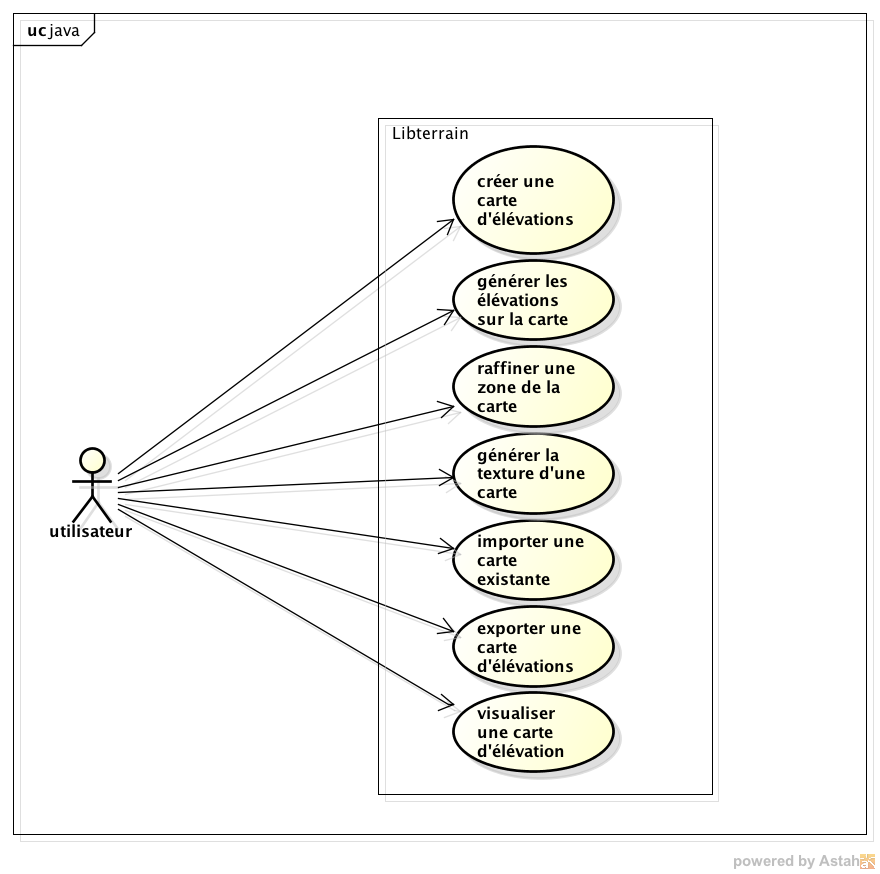
\includegraphics[width=15cm]{resources/use-case.png}
        \label{fig:use_case}
        \caption{Scénario d'exécution}
    \end{center}
\end{figure}


%Pour éviter la numérotation du sommaire
\thispagestyle{empty}
